\documentclass[a4paper,12pt,titlepage]{article}
\usepackage[french]{babel}
\usepackage[utf8]{inputenc}
\usepackage{graphicx}
\usepackage{tocloft}
\usepackage[a4paper, margin=2cm]{geometry}
\usepackage{makecell}
\usepackage{xcolor}
\usepackage{listings}
\usepackage[T1]{fontenc}
\usepackage{hyperref}
\usepackage{float}
\hypersetup{
colorlinks=true,
linkcolor=blue,
filecolor=magenta,
urlcolor=cyan,
}

% Configuration du bloc de code
\lstdefinestyle{codeStyle}{
  backgroundcolor=\color{lightgray!20},
  basicstyle=\small\ttfamily,
  breaklines=true,
  keywordstyle=\color{blue},
  language=SPARQL,
  frame=single,
  numbers=left,
  numberstyle=\tiny\color{gray},
  commentstyle=\color{gray},
  morecomment=[l]{\#}
}

\lstdefinestyle{resultStyle}{
    backgroundcolor=\color{lightgray!20},
    basicstyle=\small\ttfamily,
    breaklines=true,
    frame=single,
    numberstyle=\tiny\color{gray},
    commentstyle=\color{gray},
}

\geometry{a4paper, margin=2.5cm}

\setlength{\parskip}{10pt}

\title{Projet Knowledge Management \\ \begin{center}
    
\includegraphics[width=6cm]{../images/logo.png}
\end{center}}

\author{LAVEDER Mark-Ylann \\ \href{https://github.com/LavederMark-Ylann/SEC201}{Lien vers le dépôt GitHub}}

\date{18/06/2022}

\begin{document}

\maketitle
\thispagestyle{empty}
\clearpage

\renewcommand{\contentsname}{Sommaire}
\tableofcontents
\thispagestyle{empty}
\clearpage

\listoffigures
\thispagestyle{empty}
\clearpage


\pagenumbering{arabic}
\setcounter{page}{1}
\section{Choix du domaine}
J'ai choisi le domaine de la relation client-serveur car il s'agit d'un de mes champ d'action dans mon travail quotidien.
Etant employé comme apprenti ingénieur DevOps, je suis amené à travailler et à résoudre des problématiques sur les deux plans.

\noindent
Le contexte de mon entreprise n'a pas été retenu et seules quelques technologies sont citées.

\section{Taxonomie}
\begin{figure}[H]
    \centering
    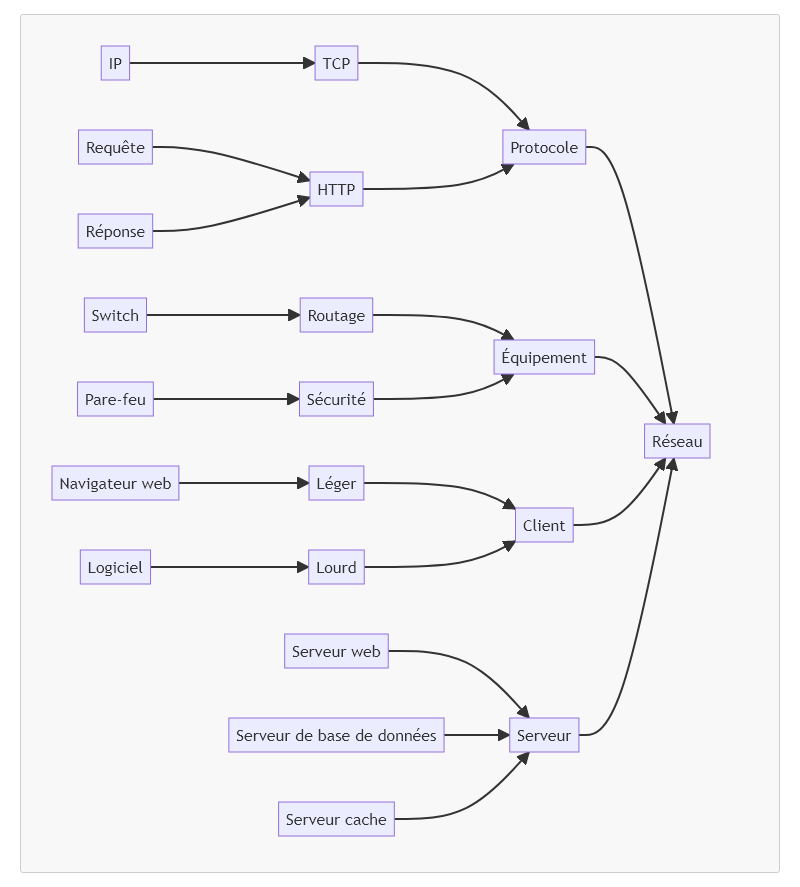
\includegraphics[width=\textwidth, height=\dimexpr\textheight-10cm\relax, keepaspectratio]{../images/mermaid_v1.png}
    \caption{Taxonomie simplifiée d'une relation client-serveur}\label{fig:Schéma de la taxonomie}
\end{figure}

\section{Ajout d'instances}

\subsection{Réseau}
\begin{itemize}
    \item IP : IPv4, IPv6
    \item Requête : GET, POST
    \item Réponse : 200, 404
\end{itemize}

\subsection{Client}
\begin{itemize}
    \item Navigateur : Chrome, Firefox
\end{itemize}

\subsection{Serveur}
\begin{itemize}
    \item Serveur Web : Nginx, IIS
    \item Serveur de base de données : MySQL, SQLServer
    \item Serveur cache : Redis, Memcached
\end{itemize}

\section{Ajout de prédicats}
\begin{figure}[H]
    \centering
    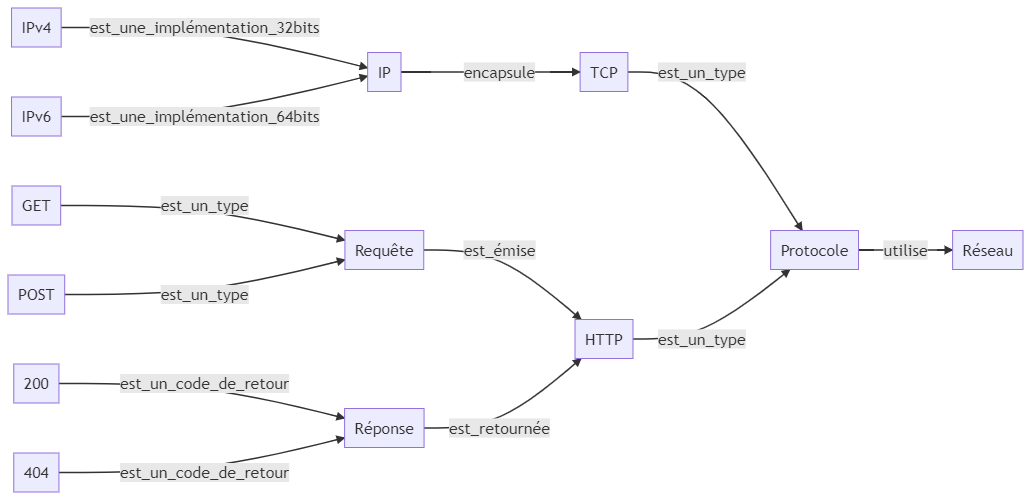
\includegraphics[width=\textwidth, height=\textheight, keepaspectratio]{../images/mermaid_v2_sub.png}
    \caption{Sous-graphe de la taxonomie simplifiée}\label{fig:Sous-graphe référençant les prédicats}
\end{figure}

\newpage
\section{Changements additionnels}
La représentation graphique de la taxonomie comporte des prédicats entre tous les noeuds.
\begin{figure}[H]
    \centering
    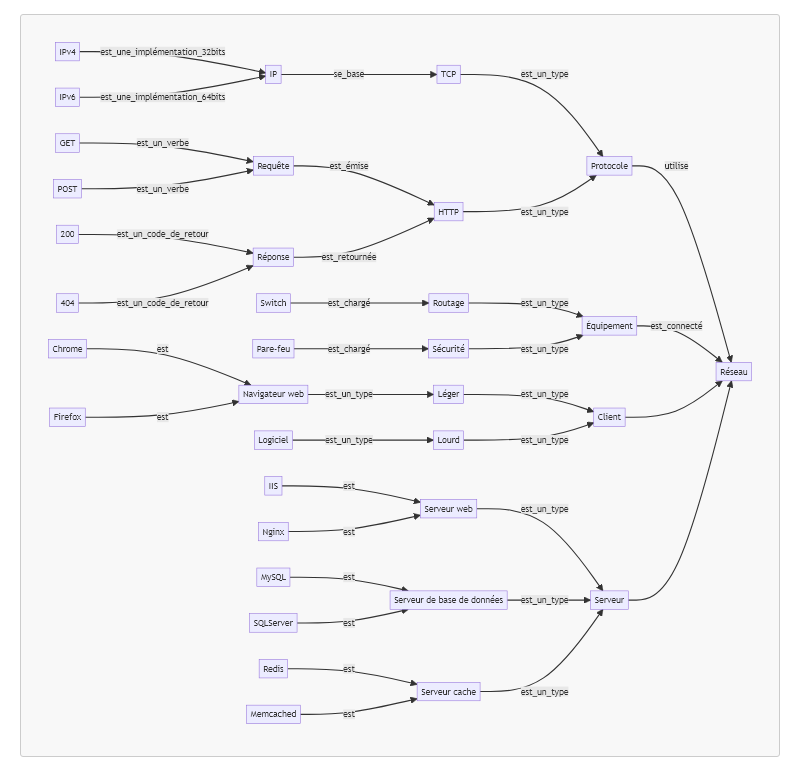
\includegraphics[width=\textwidth, height=\textheight, keepaspectratio]{../images/mermaid_v3.png}
    \caption{Graphe de la taxonomie mis à jour}\label{fig:Graphe de la taxonomie avec tous les prédicats}
\end{figure}

Ecriture en Turtle de la taxonomie.

Transformation des instances 200 et 404 en `OK` et 'Not Found' avec un lien `a un code retour'.

Ajout d'un noeud Fonction, lié à Equipement et à ses sous-classes.

\newpage
\section{Requêtes SPARQL}

\begin{tabular}{|p{0.450\textwidth}|p{0.450\textwidth}|}
  \hline
  \multicolumn{1}{|c|}{\textbf{\large{Requête}}} & \multicolumn{1}{|c|}{\textbf{\large{Résultat}}} \\
  \hline
  \multicolumn{2}{|c|}{\textbf{\large\makecell{Sélectionner les instances de ServeurWeb}}} \\
  \hline

  \begin{lstlisting}[style=codeStyle]
SELECT ?serveurWeb 
WHERE {
    ?serveurWeb rdf:type <http://example.com/ServeurWeb>.
}
\end{lstlisting}

&

  \begin{lstlisting}[style=resultStyle]
------------------------------
| serveurWeb                 |
==============================
| <http://example.com/Nginx> |
| <http://example.com/IIS>   |
------------------------------
\end{lstlisting} \\
  \hline

  \multicolumn{2}{|c|}{\textbf{\large\makecell{Décrire l'instance "Nginx"}}} \\
  \hline
  \begin{lstlisting}[style=codeStyle]
DESCRIBE <http://example.com/Nginx>
\end{lstlisting}

&
  \begin{lstlisting}[style=resultStyle]
(graph
 (triple <http://example.com/Nginx> rdf:type owl:NamedIndividual)
 (triple <http://example.com/Nginx> rdf:type <http://example.com/ServeurWeb>)
 (triple <http://example.com/Nginx> <http://example.com/version> "1.23.4")
)
\end{lstlisting} \\
  \hline

  \multicolumn{2}{|c|}{\textbf{\large\makecell{Demander s'il existe une instance de Client}}} \\
  \hline
  \begin{lstlisting}[style=codeStyle]
ASK {
    ?nav rdf:type <http://example.com/NavigateurWeb>.
}
\end{lstlisting}

&

  \begin{lstlisting}[style=resultStyle]
yes
\end{lstlisting} \\
\hline

\end{tabular}

\newpage

\begin{tabular}{|p{0.450\textwidth}|p{0.450\textwidth}|}

  \hline
  \multicolumn{2}{|c|}{\textbf{\large\makecell{Construire un graphe des ServeurWeb et leur version}}} \\
  \hline
  \begin{lstlisting}[style=codeStyle]
CONSTRUCT {
    ?serveurWeb <http://example.com/version> ?version.
}
WHERE {
    ?serveurWeb <http://example.com/version> ?version .
    ?serveurWeb rdf:type <http://example.com/ServeurWeb>.
}
\end{lstlisting}

&

  \begin{lstlisting}[style=resultStyle]
(graph
 (triple <http://example.com/Nginx> <http://example.com/version> "1.23.4")
 (triple <http://example.com/IIS> <http://example.com/version> "2.34.5")
)
\end{lstlisting}
  \\
  \hline

  \multicolumn{2}{|c|}{\textbf{\large\makecell{Insérer une nouvelle instance de ServeurWeb}}} \\
  \hline
  \begin{lstlisting}[style=codeStyle]
INSERT DATA {
    <http://example.com/Apache> rdf:type <http://example.com/ServeurWeb>.
    <http://example.com/Apache> <http://example.com/version> "3.45.6".
}
\end{lstlisting}

&

  \begin{lstlisting}[style=resultStyle]
  SPARQL update executed correctly
  \end{lstlisting}

  \\
  \hline
  \multicolumn{2}{|c|}{\textbf{\large\makecell{Supprimer une instance de ServeurWeb}}} \\
  \hline
  \begin{lstlisting}[style=codeStyle]
DELETE {
    <http://example.com/Apache> rdf:type <http://example.com/ServeurWeb>.
}
WHERE {
    <http://example.com/Nginx> rdf:type <http://example.com/ServeurWeb>.
}
\end{lstlisting}

&

\begin{lstlisting}[style=resultStyle]
  SPARQL update executed correctly
  \end{lstlisting}
  \\
  \hline
\end{tabular}

\end{document}